%    \subsubsection{Application of the Computational Image Complexity Analysis (CICA) system for facade variation complexity analysis}
%    \label{subsubsec:CICAforFacades}
%    %% description of CICA applicationnn forfacade variation modeled in blender for use in the experiment
%    %    \subsubsection{Application of the Computational Image Complexity Analysis (CICA) system for facade variation complexity analysis}
%    \label{subsubsec:CICAforFacades}
%    %% description of CICA applicationnn forfacade variation modeled in blender for use in the experiment
%    %    \subsubsection{Application of the Computational Image Complexity Analysis (CICA) system for facade variation complexity analysis}
%    \label{subsubsec:CICAforFacades}
%    %% description of CICA applicationnn forfacade variation modeled in blender for use in the experiment
%    %    \subsubsection{Application of the Computational Image Complexity Analysis (CICA) system for facade variation complexity analysis}
%    \label{subsubsec:CICAforFacades}
%    %% description of CICA applicationnn forfacade variation modeled in blender for use in the experiment
%    \input{Text/MethodologyCICAforFacades.tex}

The second essential component of the VR system is the application of the Computational Image Complexity Analysis (CICA) system, responsible for assessing the complexity of the facade variations generated within the '3D modeling' component.

To ensure a seamless evaluation of complexity and the selection of facade variations, the CICA system script is customized for integration into the Blender (v3.6) environment, streamlining the overall process.

Subsequently, the complexity scores for each of the ten selected variations within each pattern are visualized through three distinct scatter graphs, enhancing data visualization and facilitating variation comparison.
These graphs are seamlessly integrated into the VR system interface, providing participants with access to quantitative metrics within the scoring system.

Figure\ref{fig:complexitygraphRender} presents an illustrative example, combining the complexity analysis report for all three patterns using the CICA system.

For a comprehensive understanding of the workflow and functionality of the Computational Image Complexity Analysis (CICA) system for evaluating the complexity of the facade variations, a detailed flowchart is provided in Figure \ref{fig:ImageComplexityAnalysisFlowchart}, which can be found in section \ref{subsec:Image Complexity analysis}.

%% Figure of Complexity graph
     \begin{figure*}[!htb]
          \centering
          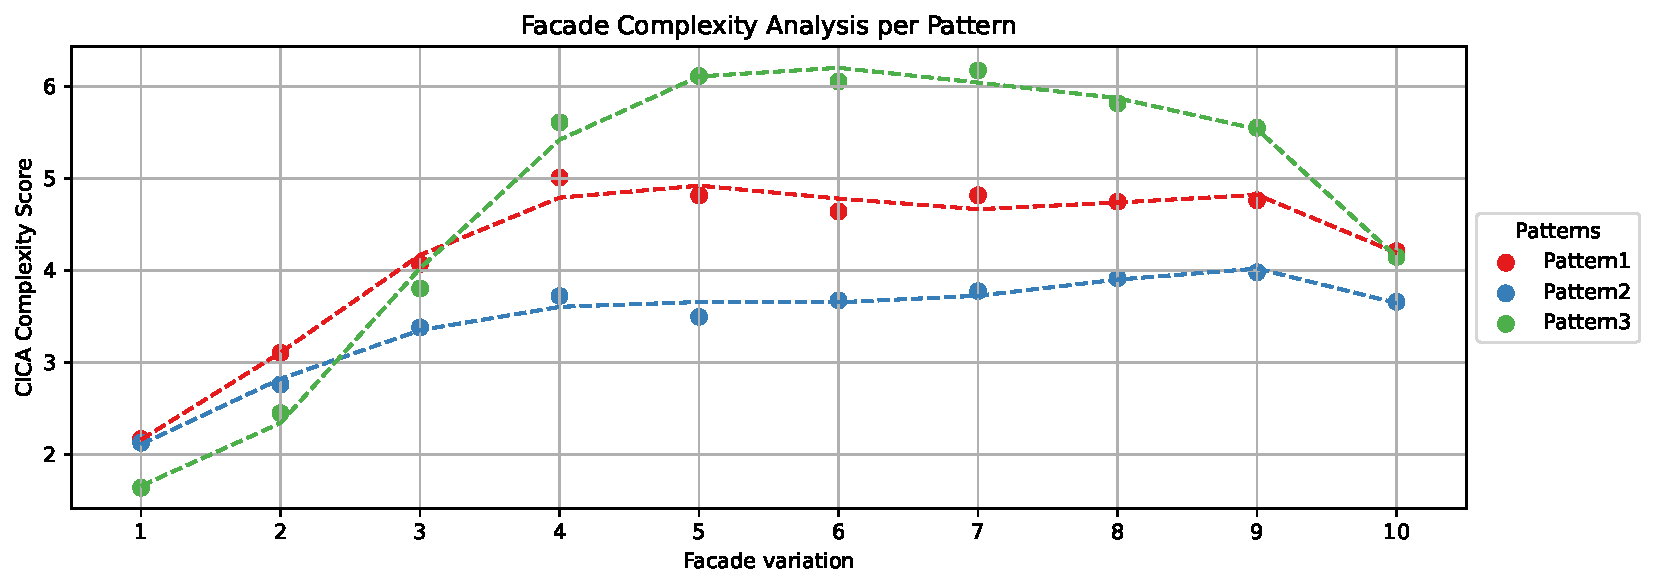
\includegraphics[width= \linewidth]{Graphs/complexitygraphrender}
          \caption{Scatter graph showcasing quantitative Computational Image Complexity Analysis scores for the rendering images of the 10 variations for each of the three patterns modeled in Blender, with an overlaid trendline highlighting the complexity level trend towards increased complexity.}
          \label{fig:complexitygraphRender}
        \end{figure*}

The second essential component of the VR system is the application of the Computational Image Complexity Analysis (CICA) system, responsible for assessing the complexity of the facade variations generated within the '3D modeling' component.

To ensure a seamless evaluation of complexity and the selection of facade variations, the CICA system script is customized for integration into the Blender (v3.6) environment, streamlining the overall process.

Subsequently, the complexity scores for each of the ten selected variations within each pattern are visualized through three distinct scatter graphs, enhancing data visualization and facilitating variation comparison.
These graphs are seamlessly integrated into the VR system interface, providing participants with access to quantitative metrics within the scoring system.

Figure\ref{fig:complexitygraphRender} presents an illustrative example, combining the complexity analysis report for all three patterns using the CICA system.

For a comprehensive understanding of the workflow and functionality of the Computational Image Complexity Analysis (CICA) system for evaluating the complexity of the facade variations, a detailed flowchart is provided in Figure \ref{fig:ImageComplexityAnalysisFlowchart}, which can be found in section \ref{subsec:Image Complexity analysis}.

%% Figure of Complexity graph
     \begin{figure*}[!htb]
          \centering
          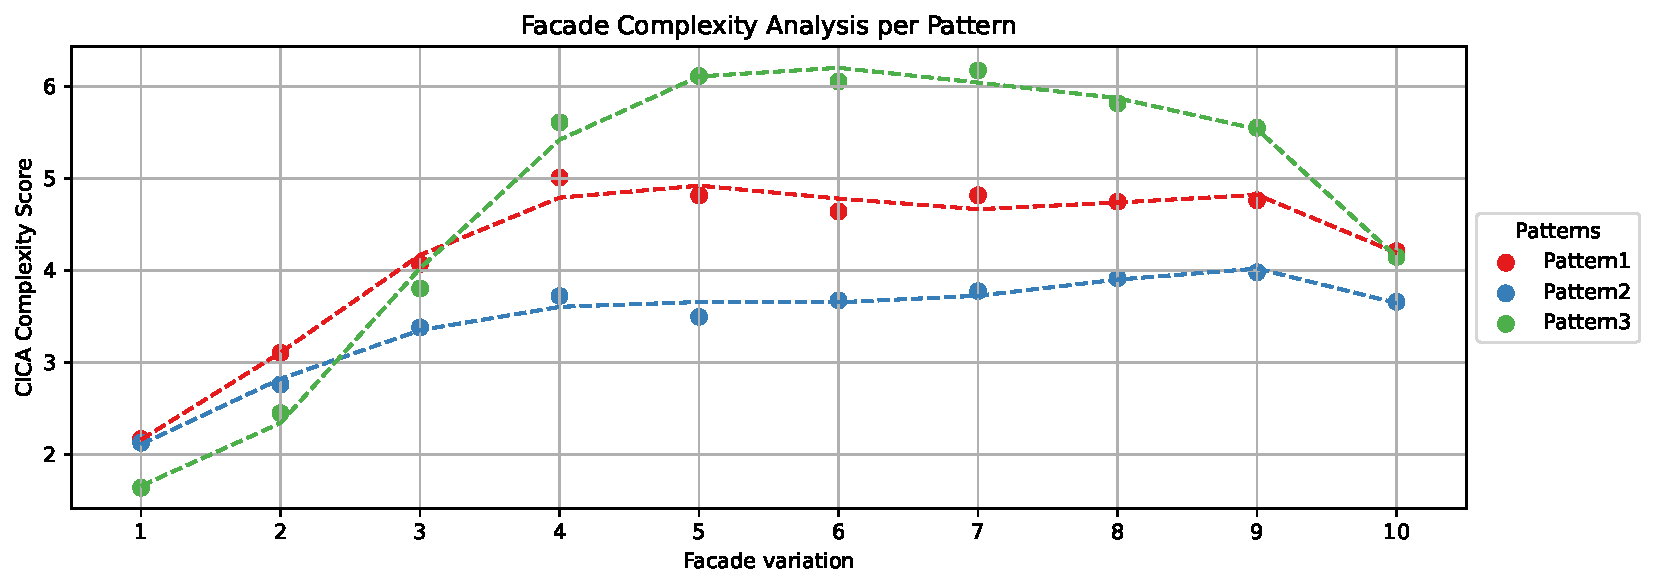
\includegraphics[width= \linewidth]{Graphs/complexitygraphrender}
          \caption{Scatter graph showcasing quantitative Computational Image Complexity Analysis scores for the rendering images of the 10 variations for each of the three patterns modeled in Blender, with an overlaid trendline highlighting the complexity level trend towards increased complexity.}
          \label{fig:complexitygraphRender}
        \end{figure*}

The second essential component of the VR system is the application of the Computational Image Complexity Analysis (CICA) system, responsible for assessing the complexity of the facade variations generated within the '3D modeling' component.

To ensure a seamless evaluation of complexity and the selection of facade variations, the CICA system script is customized for integration into the Blender (v3.6) environment, streamlining the overall process.

Subsequently, the complexity scores for each of the ten selected variations within each pattern are visualized through three distinct scatter graphs, enhancing data visualization and facilitating variation comparison.
These graphs are seamlessly integrated into the VR system interface, providing participants with access to quantitative metrics within the scoring system.

Figure\ref{fig:complexitygraphRender} presents an illustrative example, combining the complexity analysis report for all three patterns using the CICA system.

For a comprehensive understanding of the workflow and functionality of the Computational Image Complexity Analysis (CICA) system for evaluating the complexity of the facade variations, a detailed flowchart is provided in Figure \ref{fig:ImageComplexityAnalysisFlowchart}, which can be found in section \ref{subsec:Image Complexity analysis}.

%% Figure of Complexity graph
     \begin{figure*}[!htb]
          \centering
          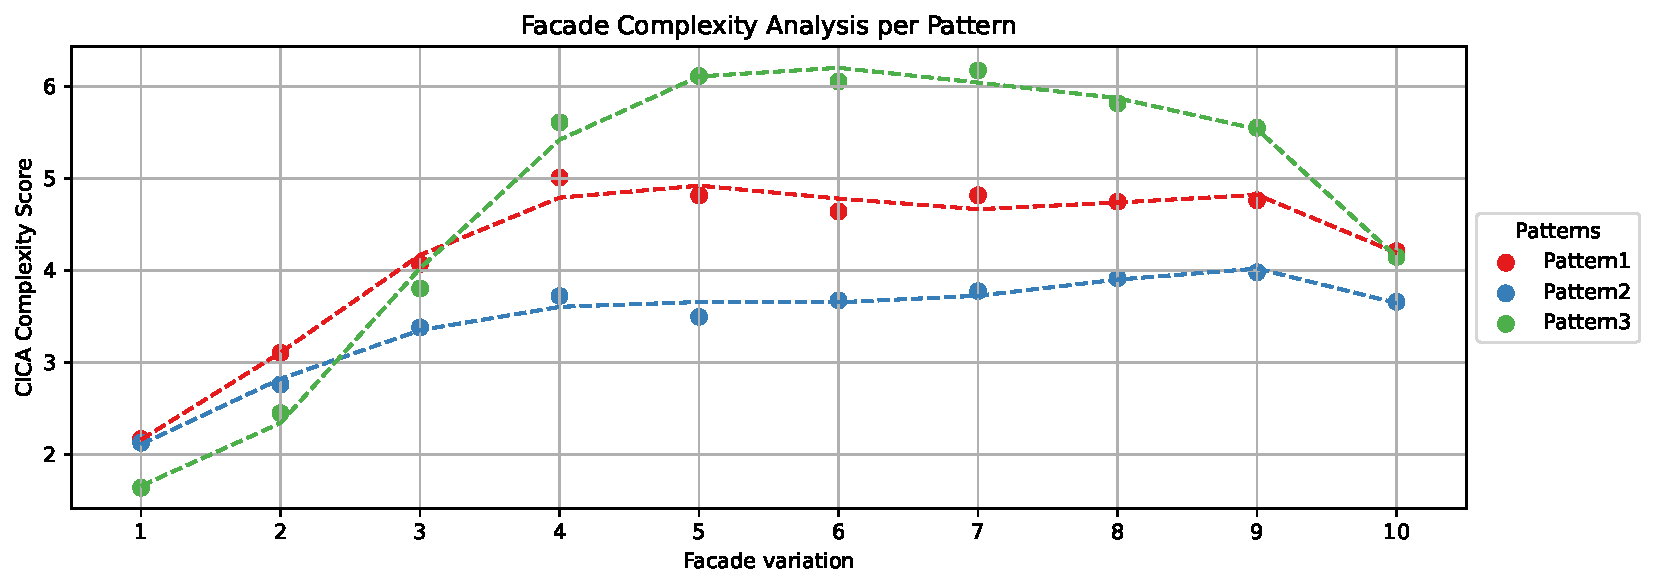
\includegraphics[width= \linewidth]{Graphs/complexitygraphrender}
          \caption{Scatter graph showcasing quantitative Computational Image Complexity Analysis scores for the rendering images of the 10 variations for each of the three patterns modeled in Blender, with an overlaid trendline highlighting the complexity level trend towards increased complexity.}
          \label{fig:complexitygraphRender}
        \end{figure*}

The second essential component of the VR system is the application of the Computational Image Complexity Analysis (CICA) system, responsible for assessing the complexity of the facade variations generated within the '3D modeling' component.

To ensure a seamless evaluation of complexity and the selection of facade variations, the CICA system script is customized for integration into the Blender (v3.6) environment, streamlining the overall process.

Subsequently, the complexity scores for each of the ten selected variations within each pattern are visualized through three distinct scatter graphs, enhancing data visualization and facilitating variation comparison.
These graphs are seamlessly integrated into the VR system interface, providing participants with access to quantitative metrics within the scoring system.

Figure\ref{fig:complexitygraphRender} presents an illustrative example, combining the complexity analysis report for all three patterns using the CICA system.

For a comprehensive understanding of the workflow and functionality of the Computational Image Complexity Analysis (CICA) system for evaluating the complexity of the facade variations, a detailed flowchart is provided in Figure \ref{fig:ImageComplexityAnalysisFlowchart}, which can be found in section \ref{subsec:Image Complexity analysis}.

%% Figure of Complexity graph
     \begin{figure*}[!htb]
          \centering
          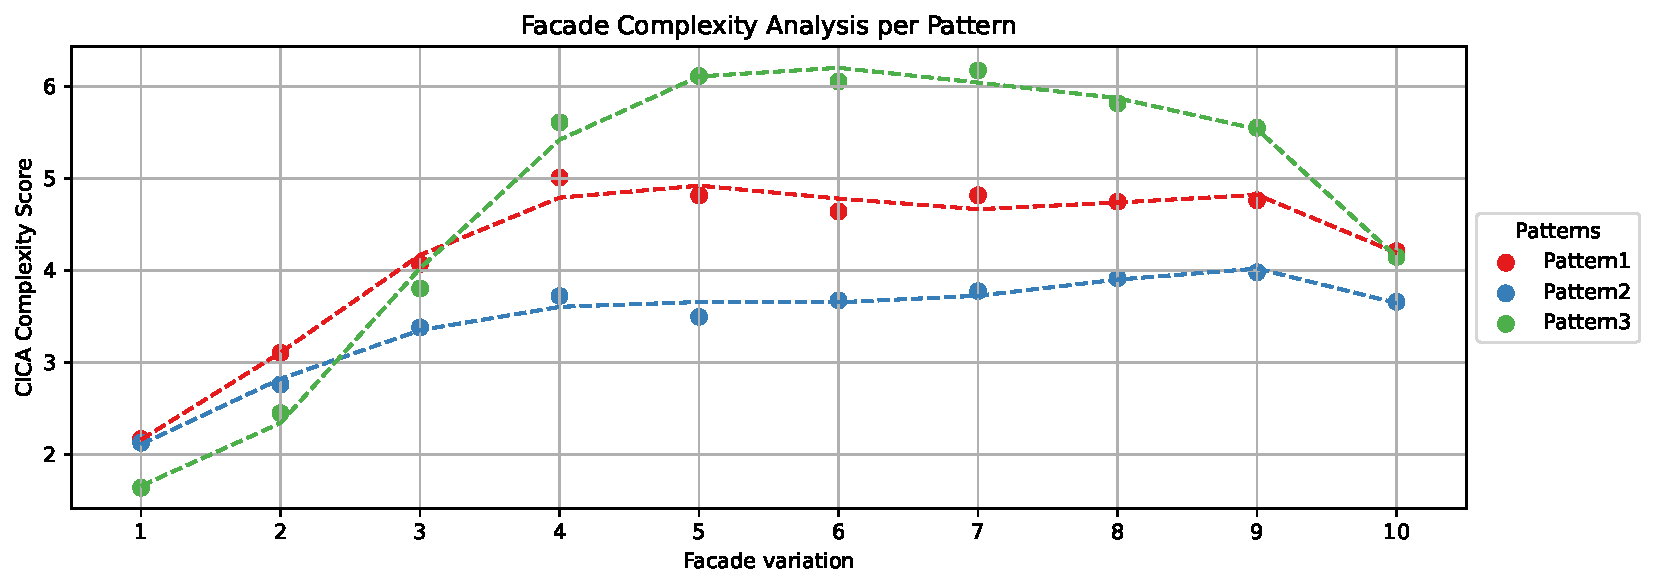
\includegraphics[width= \linewidth]{Graphs/complexitygraphrender}
          \caption{Scatter graph showcasing quantitative Computational Image Complexity Analysis scores for the rendering images of the 10 variations for each of the three patterns modeled in Blender, with an overlaid trendline highlighting the complexity level trend towards increased complexity.}
          \label{fig:complexitygraphRender}
        \end{figure*}